
\chapter{Introduction to E-Commerce and Web Analytics} % korrigiert

The focus of this thesis revolves around web performance of e-commerce websites.
Web performance can be considered a subset and specialized form of web analytics.
To provide context, this chapter provides an overview of e-commerce and web analytics.

Section \ref{section:e-commerce} provides an overview of e-commerce and explains why performance is important for e-commerce companies.

Section \ref{section:web_analytics} discusses how e-commerce companies can be audited using web analytics and what techniques and metrics are available.

Once context is provided, this thesis takes a step further and dives into web performance in chapter \ref{chapter:web_performance}.


% ---------------------------------------------------------------------------------------------------------


\section{E-Commerce} % korrigiert
\label{section:e-commerce}

This section gives an introduction to e-commerce.
Before going into the details, the emergence of e-commerce is described, starting with the Internet in section \ref{subsection:internet}.
In the following, I will briefly discuss the history of e-commerce and its types in section \ref{subsection:ecommerce_subchapter}.
The relationship between user satisfaction and the website performance is covered in section \ref{subsection:user_satisfaction}, which then leads to the section \ref{section:web_analytics} which is about web analytics.



\subsection{The Internet: Overview} % korrigiert
\label{subsection:internet}

In the last 50 years, a new technology emerged, spread over the entire world and influenced many aspects of most peoples life.
Within the turmoil of the cold war, the United State's \textit{Advanced Research Projects Agency} (ARPA) established in 1957 a communication network to bring together universities and their researches all around the country in order to be able compete against the USSR \cite{2011Cohen}.
What started as a tool for scientific collaboration evolved half a century later into the \textit{Internet}, a global network and phenomenon, to which every user with a dedicated device has access and can contribute to.
The internet is an integral part, if not the backbone of today's everyday life.
Users of the internet use it for almost everything, from sending emails, watching television, chatting with friends, order lunch, checking the weather for the next day or renting motorized scooters.

% [Numbers]

In 2021, the internet has 4.66 billion users, which is around 60\% of the world population.\footnote{Following statistics are taken from \url{https://datareportal.com/reports/digital-2021-germany} [14.05.2021]}
Compared to 2020, the number of internet users increased by 7.3\%.
In Europe, more than 90\% of the population are internet users.
For a developed country like Germany, the numbers are even more impressing:
94\% of the German population are using the internet with an average daily time of over five hours.

Those numbers demonstrate impressive that the internet is an integral part of our daily life.
Along the rise of the internet, transactions and processes falling under the term of e-commerce are climbing as well.
Before discussing the term "e-commerce" and take a grasp at its history and types, some statistics are presented to demonstrate the importance of e-commerce.


\subsection{E-Commerce}
\label{subsection:ecommerce_subchapter}

\subsubsection{The Importance of E-Commerce} % korrigiert

From the global data report\footnote{\url{https://datareportal.com/reports/digital-2021-germany} [14.05.2021]}, one can read out that over 90\% of the world population visited an online retail site and over 76\% of the world population purchased a product online.
% For most of the categories growth is over 15\%.  % which categories ?
For or a western country like Germany, the figures are higher:
92.5\% of the German population visited an online retail site and over 80\% purchased a product online.
And the usage is expanding: the growth of the amount spent within the category food and personal care is 28.6\%, and 17.6\% for the category fashion and beauty.

E-commerce sales have grown steadily over the past 20 years, topping to 57.8 billion in 2019.\footnote{\url{https://einzelhandel.de/presse/zahlenfaktengrafiken/861-online-handel/1889-e-commerce-umsaetze} [14.05.2021]}

% [Corona: Even more growth]

The COVID-19 pandemic with its implications had and still has an not negligible impact on the growth of e-commerce.
Several measures were taken to stop the spread of the virus and the number of deaths, one of which was to minimize physical interaction between people.
This leads consequently to a shift of human interactions to the internet.
Along this, e-commerce benefits.
Bhatti et al. \cite{2020Bhatti} conclude that "e-commerce enhanced by COVID-19".



\subsubsection{Brief History of E-Commerce} % korrigiert

E-Commerce, or electronic commerce, is according to the \textit{Encyclopædia Britannica} about "maintaining relationships and conducting business transactions that include selling information, services, and goods by means of computer telecommunications networks."\footnote{\url{https://www.britannica.com/technology/e-commerce} [19.05.2021]}
In short, e-commerce is about buying and selling products and services via the internet.

The success of e-commerce is closely linked to the tremendous advances in Internet technology in recent years:
The development of the \textit{Electronic Data Interchange} (EDI) starting in the 1960s standardised the communication between two machines.
Personal computers were introduced in the 1980s, and one of the first examples of an online shop is the \textit{Electronic Mall} opened by CompuServe in 1984.
Another crucial milestone is the launch of the \textit{World Wide Web} (WWW) in 1990, which made the internet accessible to everyone.
With social media visible on the horizon from the 2000s, new possibilities for businesses and consumers alike to participate in e-commerce arise, for example, by enabling new marketing strategies or providing new sales channels.
New devices such as smart phones and tablets lowered the barrier to participate in e-commerce.
While e-commerce was available at any time, the new devices brought flexibility and mobility, making e-commerce available everywhere \cite{2019Hermogeno}.

With the continued advancement in technology, e-commerce can expect a bright future with trends such as AI recommendation systems, outstanding UX thanks to virtual reality, or even more simpler payment methods through cryptocurrencies.\footnote{\url{https://www.spiralytics.com/blog/past-present-future-ecommerce/} [19.05.2021]}


\subsubsection{Types} % korrigiert

There are several types in e-commerce and they emerge from the possible combinations between the actors \textit{Business}, \textit{Consumer} and \textit{Government} \cite{2017DosSantos}, as shown in table \ref{table:types_ecommerce}.
The research question and the context of this thesis revolve around e-commerce websites in the sense of online shopping (B2C).
B2C will be briefly discussed below, types such as C2C or C2G are not of interest and will not be considered further.

\begin{table}[h]
	\small
	\centering
	\begin{tabular}{| c | c | c | c |}
	\hline
	 & Business & Consumer & Government \\
	\hline
	Business & B2B & B2C & B2G \\
	\hline
	Consumer & \cellcolor{lightgrey} & C2C & C2G \\
	\hline
	Government & \cellcolor{lightgrey} & \cellcolor{lightgrey} & G2G \\
	\hline
	\end{tabular}
	\medskip
	\caption{Types of e-commerce.}
	\label{table:types_ecommerce}
\end{table}


\paragraph{B2C} % korrigiert

Business to Consumer in e-commerce describes basically online shopping, by means of a business offering its services and products to the consumer over the \textit{WWW}.
The consumer can browse through the products and services presented within an online shop and order them directly via the website.
A variety of payment and delivery options conclude the B2C type \cite{2020Heinemann}.
% TODO cite Heinemann with correct page p. 75 ?

%TODO where to put this sentence?
For an aspiring business, there are several ready-made software solutions for setting up an online store, as for example. \textit{Shopify}, \textit{ePages}, \textit{Magento} or \textit{WooCommerce} \cite{2019Steireif}.

A famous example of a B2C company is \textit{Amazon}.
On the 16th of July in 1995, Amazon launched as a website and entered the stock market on the 15th of May 1997 \cite{2019Stone}. % cite also that this is directly from page p. 47 ?
Amazon has been successful, with the stock starting at \$1.5, which is at around \$3200 as of this writing.\footnote{\url{https://finance.yahoo.com/quote/AMZN?p=AMZN} [19.05.2021]}
Today, Amazon employs over 1 million people\footnote{\url{https://www.statista.com/statistics/234488/number-of-amazon-employees/} [19.05.2021]} and serves the desires of 200 million paying prime members.\footnote{\url{https://www.statista.com/statistics/829113/number-of-paying-amazon-prime-members/} [20.05.2021]}
\\

% [Pro and Con]

By taking a quick look at the pros and cons of an online store, it becomes clear that some of the advantages are that: there is no need of a real, physical store to showcase and sell the products; the virtual shop is available to the consumer at any time and has no closing hours; there is a high potential for the online shop as it is part of growing market; online business is scalable; due to tracking algorithms, precise targeting as well as data analysis is possible; to start an online business, there is not so much floating required and there are generally lower costs; it is possible to provide a personalized customer experience.

Some disadvantages are that the speed of market is rapid, competitors arise everyday everywhere and technology evolves quickly while consumers expectations go high \cite{2019Hermogeno}, \cite{2020Lang}.
\\

% [Performance of online shop is important]

Another disadvantage is that there is no direct or physical connection with the consumer.
As described above, online shopping takes place on the virtual WWW, i.e. personal interaction between buyer and seller is not possible and the shopping experience takes place on a website, from which it follows that the overall virtual user experience must be excellent in order to compete.

In the next section, I will describe the findings between the correlation between user satisfaction and the performance of the retailers web presence.


% ------------------------------------------


\subsection{User Satisfaction and Performance in E-Commerce} % korrgiert
\label{subsection:user_satisfaction}

% [User Satisfaction]

The aim of this thesis is not to deep dive into terms and concepts or the non-trivial problem of defining user satisfaction, usability or the like.
Therefore the term user satisfaction is in this context loosely defined as how happy the user is with the website he or she interacts with.\footnote{For a discussion see "User satisfaction measurement" in \cite{2010Islam}}

% [Performance]

Performance can be understood as the speed of an online shop, e.g. how long it takes the page to load, how quickly the user can interact with the page, and how the user perceives the performance of the website.
In section \ref{section:measurement_methods} I will discuss that measuring performance is not so trivial and there are a lot of ideas and metrics to measure it (section \ref{section:web_performance_metrics}).


\subsubsection{Studies about User Satisfaction and Performance}

% A plethora of information and studies about the phenomenon of user satisfaction and website performance is collected at \textit{SpeedHub.org}, a portal by \textit{Baqend} in cooperation with \textit{Google} which provides "the largest systematic study of Mobile Site Speed and the Impact on E-Commerce."\footnote{\url{https://www.speedhub.org/} [21.05.2021]}
% Not only are studies and reports available on the hub, but also collections of videos and blog posts.

% [code.talks 2019]
% In his talk at code.talks 2019, Felix Gessert summarizes the results and provides insights into the most important aspects and questions of the study so far \cite{2019Gessert}:

% [User Profile and Psychology]

There are numerous studies that shed light on various aspects of the relationship between user satisfaction and performance.
A selection is summarized here.

Unbounce \cite{2019Thinkfast} and Awwwards, in partnership with Google \cite{2017Brainfood}, offer insights into user profiles.
In terms of gender, young women are the most demanding consumers and are less likely to buy from slow sites.
In general, people between the ages of 18 and 24 have higher expectations of a site's speed than their older counterparts.
There are also differences between nations and regions, for example people from Japan have the highest expectations, which is almost certainly related to technological advancements in that country.
% Not only the expectations themselves differ geographically, but also how speed influences the users, for example "speed influences New Yorkers more than Californians."

% In terms of performance, researchers generally suggest keeping wait times below one second to keep users' attention. (see "Performance perception" in \ref{section:web_performance_introduction}). 

% [Devices]

DeviceAtlas \cite{2019Deviceatlas} provides insights into devices in use.
Their studies show that mobile users are more likely to buy products and services than their colleagues using a desktop computer, where iOS users have generally more expectations regarding site speed.
 
% [Context]

Akamai \cite{2014Akamai} offers insights into psychological aspects of user satisfaction and performance.
Their observations show that relaxed and calm users perceive pages faster than stressed or hurried users.
Also users experience websites more slowly while on the go.

% [Studies]

There are many other real world examples and studies that prove and demonstrate the importance of website speed in terms of user satisfaction and ultimately sales:
\textit{Amazon} \cite{2006Linden} found out that a decrease of 100 ms in page loading leads to -1\% conversion rates.
If the site loads 100 ms faster, \textit{Walmart} \cite{2012Walmart} observed that the revenue increases by 1\%.
For \textit{Zalando} \cite{2018Zalando}, increasing site speed by 100 ms has led to an uplift of 0.7\% revenue per session.


% [SEO]

Search engine optimization is heavily impacted by load speed:
For \textit{Google} \cite{2006Mayer}, 500 ms slower sites led to a decrease of 20\% in traffic.
\textit{GQs} \cite{2015GQ} traffic increased by 80\% after the page load went down from 7 s to 2 s.
And for \textit{Pinterest} \cite{2017Pinterest}, 40\% faster loads led to 15\% more SEO traffic.


% [Engagement & Satisfaction]

User engagement and satisfaction also depend heavily on loading times:
\textit{Forrester} \cite{2017Forrester} noted an increase of 60\% for the session length while brining down the load time by 80\%.
\textit{Akamai} \cite{2017Akamai} monitored that the bounce rate climbed up incredible 103\% when the load time increased by 2 seconds.
And for the \textit{AberdeedGroup} \cite{2008Aberdeen}, the customer satisfaction dropped by 16\% at one more second delay in response times.

In summary, it can be said that many studies and practical examples prove and demonstrate that faster websites and online stores lead to a better user experience and usually to happier customers.
In commercial terms, one can conclude that page speed equals money.
\\

In order to properly test the effects of performance on users, a scientific method is required.
A/B testing as a controlled experiment is one of them and will be explained in the next section.
After discussing A/B testing, I will move on to examining \textit{Web Analytics}, a term that encompasses methods, tools, and instruments for companies to better understand their business and customers.


\subsubsection{A/B Testing} % korrgiert

Controlled experiments like A/B testing are not a new tool for scientists and researchers and were used as early as the 1920s \cite{2016Kohavi}.
With the advent of the Internet in the 1990s, the concept was adopted into the online domain and is now used by large companies such as Amazon, Facebook or Google to test ideas and hypotheses directly on a live system.
Controlled experiments such as A/B testing are used to aid decision making and provide a "causal relationship with high probability" \cite{2016Kohavi}.
They enable a data-driven and quantitative validation of the hypothesis \cite{2018Morys}.

Controlled experiments help to test hypothesis and questions of form: "If I change feature X, will it help to improve the key performance indicator Y?"

To answer this question,  two systems are needed: \textit{Version A}, the control variant or default version, and a slightly different \textit{Version B,} called the treatment.
If more than two versions or one treatment should be evaluated at the same time,  an A/B/n split test has to be implemented.
With a univariable setup, only one variable differs between the systems; with a multivariable structure, several variables are changed at the same time.

Usually, the users of the system are randomly split into two groups and testing is directly performed with real users on a production system.
It is advantageous, also compared to other experimental set-ups, that the users and participants are not aware that they are part of an experiment, which leads to fewer biases and side effects.
In order to measure the differences and the user behaviour, web analytics has to be integrated within the system \cite{2016Kohavi}.

%TODO add some stuff from Heinemann 2020 A/B Tests nach 4.1.4 ?

A brief and general discussion of controlled experiments in computer science can be found in chapter X.  
\\

% [Transition to Web Analytics]

To continue with the question of performance and user satisfaction, A/B testing allows two different versions of the same site to be served to two groups at the same time, one site being slow and the other being fast, without users knowing.

An implemented web analytics system makes it possible to measure how the various systems and user groups behave.
What web analytics exactly is, what tools are available and what a web analytics process looks like, is discussed in the next section.



% TODO write those steps down ?
% 2018 Morys
%- 5 steps:
%- 1. quality of hypothesis according to SOR Paradigma
%- 2. quality of testconcept: isolation and contrast of changed parameters
%- 3. quality of implementation and quality assurance: running tests should not be visible by user (e.g. suddenly UI changes) and performance of website should not be impacted
%- 4. quality of measurement: significant difference in primary goals
%- 5. quality of statistical interpretation: amount of data, statistical methods

% 2012 Kessler 17.2  AB Tests ?


% -------------------------------------------------------------------------------------------
% -------------------------------------------------------------------------------------------


\section{Web Analytics} % korrigiert
\label{section:web_analytics}

This section is about web analytics.
I will first discuss definitions and give a short introduction to web analytics in section \ref{subsection:web_analytics_introduction}.
Then, a brief history of web analytics will be given in section \ref{subsection:web_analytics_history} to help contextualize.
After describing how web analytics can be applied in practice in section \ref{subsection:web_analytics_practice}, section \ref{subsection:web_analytics_logfile_pagetagging} discusses methods for data collection.
Finally, section \ref{subsection:web_analytics_metrics} discusses metrics used in web analytics.


\subsection{Introduction to Web Analytics} % korrigiert
\label{subsection:web_analytics_introduction}

% [Definitions]
What is \textit{Web Analytics}?
A review of the literature shows that there are several definitions:

Nakatani et al. state that "Web analytics is used to understand online customers and their behaviors, design actions influential to them, and ultimately foster behaviors beneficial to the business and achieve the organization's goal" \cite{2011Nakatani}.
According to this definition, web analytics is about gaining insight into the users of the system, not only who or what they are, but also how they interact with the system.
In addition, the definition emphasizes that the underlying motivation of web analytics is to achieve business goals.

Singal et al. provide a more technical definition by pointing out that "Web Analytics is the objective tracking, collection, measurement, reporting and analysis of quantitative internet data to optimize websites and web marketing initiatives" \cite{2014Singal}.
Again, the ultimate goal is to drive business, but using data science methods and tools, such as big data tracking, collection and analysis.

Bekavac et al. provide a similar definition by pointing out that web analytics is "the analysis of qualitative and quantitative data on the website in order to continuously improve the online experience of visitors, which leads to more efficient and effective realization of the company's planned goals" \cite{2015Bekavac}.

% TODO: where can i find this officially ?
% Official definition by WAA: the measurement, collection, analysis and reporting of Internet data for the purposes of understanding and optimizing Web usage.

% TODO add 2009 Waisberg? "Web Analytics can be defined as the act of increasing a website’s persuasion and relevancy to achieve higher conversion rates."

% TODO add Croll 2009? "Today, web analytics is a marketing discipline used to measure the effectiveness of communications strategies" p.83

% [Use Cases]

Zheng et al. describe four main use cases for web analytics \cite{2015Zheng}:

\begin{itemize}
\item Improving the overall design and usability, for example of the navigation or layout of the website.
\item Optimize for your business goals: Whatever goals the business is trying to achieve, generating conversions is the goal.
\item Monitor campaigns: Understand and measure the success of advertising campaigns.
\item Improve performance by examining metrics such as page load time.
% This is discussed further in chapter \ref{chapter:web_performance}.
\end{itemize}

Summarizing the above definitions, it is noticeable that web analytics consists of two important elements: a data-driven, information-oriented and technical element of collecting and analysing data about users, and a commercial and business-oriented element that provides the main motivation for collecting the data primarily by setting business goals.


% [Challenges]

Web analytics can also be complex, and there are some obstacles and challenges to overcome.
Kumar et al. describe some of the hurdles as follows \cite{2019Kumar}:
The analysis and interpretation of the data and the goals and measures derived from it are reactive rather than anticipatory, since "predictive modelling applications" for web analytics are not yet on the market.

Big data, that is the volume, variety and velocity of data collected, can be challenging to manage,
for example, important insights can be lost or overlooked.

Privacy and the information collected from visitors and customers can be another challenge in terms of inappropriate use of data and GDPR compliance.



% ------------------------------------------


\subsection{Brief History of Web Analytics} % korrigiert
\label{subsection:web_analytics_history}

The history of web analytics can be described as a transformation from an IT domain and a technical log file analysis tool to a sophisticated, polymorphic tool for marketers.

% [For IT: Logs]

Each time a user requests an HTML file or other resource from a web server, the server makes an entry in a special log file \cite{2014Singal}.
The first log entries followed the \textit{Common Log Format} (CLF) which provides rudimentary information such as the date, the HTTP status code or the number of bytes transmitted.
In 1996, the \textit{Extended Log Format} (ELF) was introduced with more flexibility and information in mind.
Thanks to the standardized format of the log files, it was possible to create software that evaluates the log files and presents them to users in a readable form.
\textit{GetStats} was one of the first tools which generated statistics and user friendly output for analysts \cite{2009Croll}. % add p. 69?
In 1995, Dr. Stephen Turner developed \textit{Analog}, the first free software for analysing log files \cite{2015Zheng}.
Log file analysis will be further discussed in section \ref{subsubsection:log_file}.

% [Shift]

What was initially mainly interesting for maintenance and IT staff, who for example answered the question of how many 404s occurred on the server, developed into an interesting website information pool for marketers.

As the available information increased, it became clear that the data could be used for more than just analysing server behaviour.
But log file analysis was not enough to provide details about how users interact with the site.
Web analytics underwent a transformation from log analysis to user data tracking, analysis, and reporting.

Croll \cite{2009Croll} describes the move of analytics from IT to marketing with three steps:

\begin{enumerate}
\item JavaScript eliminated the need for log files and enabled marketers to maintain and deploy their analytics solutions themselves, making them less dependent on IT.
\item The introduced advertising economy of search engines like Google led to a new focus of analysts on user attraction and conversion rates.
\item New cost models allowed marketers to pay for the analytics service based on website traffic, rather than paying upfront for hardware and software. Analytics spend was thus linked to website traffic and, ideally, revenue.
\end{enumerate}

% [For Marketing: JS]

In 1990 the WWW started and in 1993 one of the first widely used browsers \textit{Mosaic} was launched.
At the same time \textit{WebTrends} developed and released one of the first analytics software.
A lot more services followed, such as \textit{WebSideStory} in 1996 \cite{2009Croll}
or \textit{Quantified} by Urchin in the same year \cite{2009Croll}.

Page tagging made it possible to collect not only technical data, but also business-relevant information.
Visitors and their behaviour were the focus, shaping questions like: How is this user behaviour related to a purchase? If a user buys shoes, will he also buy socks?
The development and implementation of cookies enabled the identification of unique users.
Not only business-relevant questions were asked and answered, but also studies on performance and usability \cite{2009Croll}. % add p. 69 ?
More details about page tagging can be found in section \ref{subsubsection:page_tagging}.
\\

% [WAA, Today]

In 2003, Edwards, Eisenberg and Sterne founded the \textit{Web Analytics Association} (WAA).
The WAA brings together and supports all the players in web analytics such as users, marketers and IT specialists on an international stage.
Due to digitalization and its all-encompassing effects, the WAA has renamed itself \textit{Digital Analytics Association} (DAA) in 2012 because the web is not the only area where users leave their digital footprint \cite{2014Singal}.

As described in the section above, participant and user numbers on the Internet continue to rise and now all Fortune 500 companies operate websites, with web analytics a key marketing tool \cite{2019Kumar}.

Some of the most established tools today are \textit{Google Analytics}, \textit{Adobe SiteCatalyst}, \textit{Webtrekk} and \textit{Piwik} \cite{2020Heinemann}. %  add chapter 4.1.4 ?
Google Analytics will be further discussed in section \ref{subsection:google_analytics}.

% [Future]

Looking ahead, Zheng et al. identify several trends for web analytics, such as mobile web and application-specific analytics like video, search, learning, or social media analytics \cite{2015Zheng}.


% TODO next section will be about process ??

% TODO add Image: Genesis of Web Analytics (nice graphic) with WAA, DAA ? should remove then in-page analytics arrow

% TODO add somewhere Some methods about tool selection are described in chapter X.


% ------------------------------------------


\subsection{Web Analytics in Practice} % korrigiert
\label{subsection:web_analytics_practice}

Web analytics can be described as a process in which the main goal is usually to increase sales.
The literature cites two main ideas and processes, the first from the Web Analytics Association and the second from industry best practices.
They are briefly described in this section.

Both processes have in common that they are aimed at improving the website and thus increasing business revenue.

% [KPIs]

\textit{Key Performance Indicators} (KPIs) are the ideal tool for the instrumentation of web analytics and help to identify areas and potential for improvement.
They are an integral part and play an important role in any web analytics process as they provide a "in-depth picture of visitor behavior on a site" \cite{2009Jansen}. % add ch. 6.2 ?

KPIs can differ depending on the business in which they operate.
For commercial domains, common KPIs are conversion rates, average order or visit value, customer loyalty, bounce rate, etc. \cite{2014Singal}.

Defining the right KPIs and aligning them with business goals is a critical step in any web analytics process.

% TODO add more ?:
% 2015 Bekavac:  KPIs for commercial model: Ratio of new to returning visitors, percentage of new visitors, referring domains, search keywords/phrases, average order value, key conversion rates


\subsubsection{WAA Process Guide} % korrigiert

% TODO compare both processes directly with a table with 2 columns?

The Web Analytics Association offers a web analytics guide that consists of nine steps. They are \cite{2009Jansen}: % add ch. 6.2 ?

%TODO actually i think its nicer to draw a diagram here, with boxes connected with arrows. Will also take less space
\begin{enumerate}
\item Identify key stake holders
\item Define primary goals of website and prioritize them
\item Identify most important site visitors
\item Determine key performance indicators
\item Identify and implement the right solution
\item Use multiple technologies and methods
\item Make improvements iteratively
\item Hire and empower a full-time analyst
\item Establish a process of continuous improvement
\end{enumerate}


\subsubsection{Industries Best Practices} % korrigiert

On the contrary, Waisberg and Kaushik \cite{2009Waisberg} derive a five-step process from industry best practices with the main goal of improving the website and increasing sales: 

\begin{itemize}
\item Define Goals
\item Build KPIs
\item Collect Data
\item Analyse Data
\item Implement Changes
\item Repeat last two steps
\end{itemize}

% TODO add graphic instead of list ??


% [Comparison]

When comparing the two proposed processes, it becomes clear that both focus on identifying and being aware of the most important business goals.
The WAA process is a finer-grained and more practical approach, with Waisberg and Kaushik abstracting the main activities.


% ------------------------------------------


\subsection{Data Collection: Log File Analysis and Page Tagging} % korrigiert
\label{subsection:web_analytics_logfile_pagetagging}

There are four main methods of collecting data for web analytics: through log file analysis, JavaScript page tagging, web beacons, and packet sniffing \cite{2009Waisberg}.

As mentioned in section \ref{subsection:web_analytics_history}, the two main methods of data collection are log file analysis and page tagging.
In this section I will briefly describe and compare both mechanisms.


\subsubsection{Log File Analysis} % korrigiert
\label{subsubsection:log_file}

As described earlier, log file analysis is about gaining insights from the log file records of the web server.
Log file analysis is considered the traditional and original approach to web analytics \cite{2011Marek}, \cite{2015Zheng}.
Once the user types a URL into the browser and presses enter, the request is forwarded to a web server.
The server then creates an entry in a log file and sends the requested page or resource back to the client as a response \cite{2009Waisberg}.
The information within the log entry can vary depending on the log format.
Typically, the IP, browser, timestamp, time taken, bytes transferred, whether there is a cache hit, and the referrer are specified \cite{2009Waisberg}.
The standardized Common Log format includes host, ident, authuser, date, request, status, and bytes, as shown in listing \ref{lst:log}.\footnote{\url{https://www.w3.org/Daemon/User/Config/Logging.html\#common-logfile-format} [03.06.2021]}

\begin{center}
\begin{lstlisting}[caption={CLF}, language=bash, numbers=none, basicstyle=\tiny, label={lst:log}]
127.0.0.1 user-identifier frank [10/Oct/2000:13:55:36 -0700] "GET /apache_pb.gif HTTP/1.0" 200 2326
\end{lstlisting}
\end{center}
% TODO better caption

Standard formats of log files and entries allow log file analysis software such as \textit{Analog}, \textit{Webalizer} or \textit{AWStats} to process, analyze and report valuable statistics to users \cite{2015Zheng}.

% [Pro]

Below are some points that describe the advantages and disadvantages of log file analysis.
The advantages of log file analysis are (\cite{2009Waisberg}, \cite{2011Nakatani}, \cite{2014Singal}, \cite{2015Zheng}):
%TODO just cite here above all or in the list ?

\begin{itemize}
\item JavaScript and cookies are not required on the client side
\item Maintainer of the website and server owns the data %cite 2009 Waisberg
\item Bots and web crawler requests are also logged %cite 2009 Waisberg
\item History of data is available %cite 2011 Nakatani
\item Log entries are reliable %cite 2011 Nakatani
\item The standard format of log files enables easy switching of analysis tools %cite 2011 Nakatani
\item The web server also logs failed requests %cite 2011 Nakatani
\item No modifications to the website required %cite 2015 Zheng
\item Does not demand more bandwidth %cite 2014 Singal
\end{itemize}


% [Con]

Some disadvantages of log file analysis are (\cite{2011Marek}, \cite{2015Zheng}):

\begin{itemize}
\item The log entries mainly contain technical information that is not very useful for analyzing user behavior. Business-related metrics such as bounce rates are not available. % cite Marek 2011
\item Only direct requests from the client to the web server are logged: Any user interaction in the web browser that does not trigger a request is not logged. Responses from caches and proxies are also not visible in the web server log file. Only interactions with the web server are logged.
%cite 2015 Zheng
\end{itemize}


% ------------------------------------------

\subsubsection{Page Tagging} % korrigiert
\label{subsubsection:page_tagging}

In a nutshell, page tagging describes the analytics method where JavaScript is embedded into the website that collects data and sends it to an analytics server \cite{2011Marek}.
For this purpose, JavaScript must be integrated on each page to be analysed \cite{2009Waisberg}.
Page tagging is the most important method of web analytics today \cite{2015Zheng}.

Croll provides a illustration (figure \ref{figure:page_tagging}) of the page tagging process, which is explained below \cite{2009Croll}.

\begin{figure}[h!]
\begin{center}
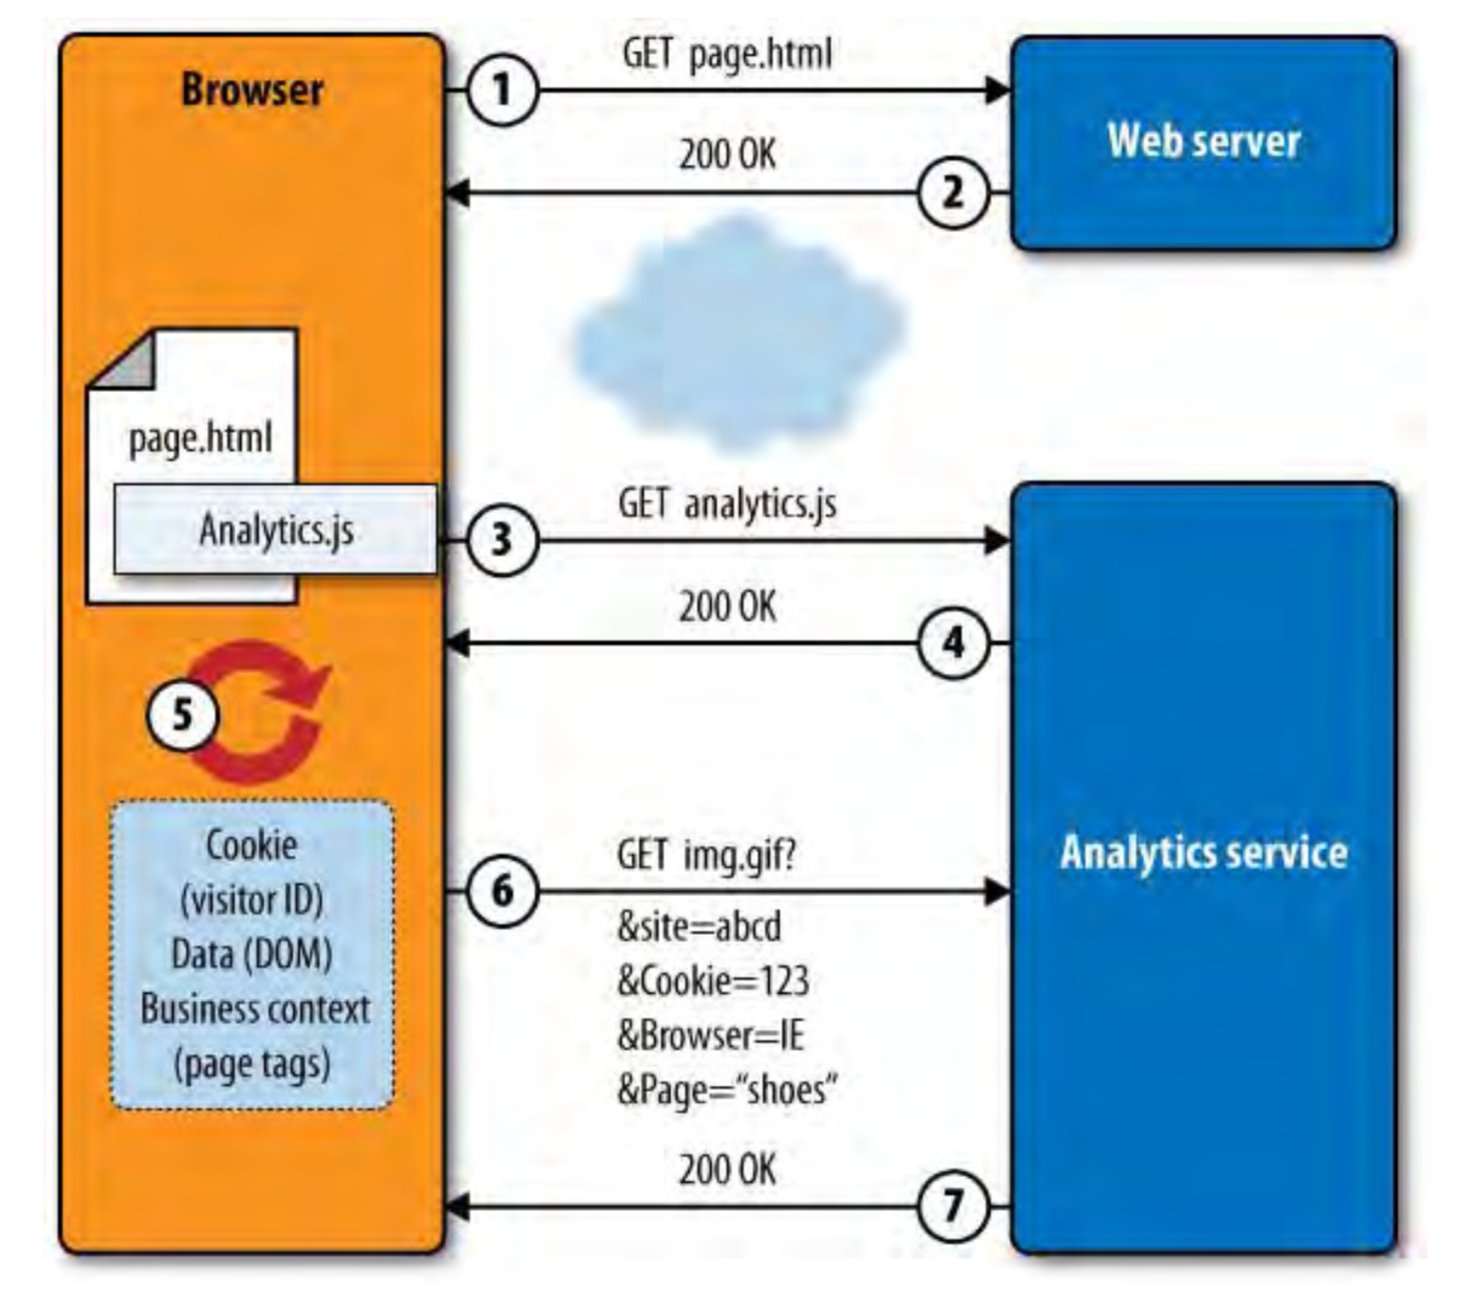
\includegraphics[width=0.5\textwidth]{page_tagging.png}
% \caption{Page Tagging, taken from \cite{2009Croll}}
\caption[Page Tagging]{Page Tagging, taken from \cite{2009Croll}}
\label{figure:page_tagging}
\end{center}
\end{figure}

The client (browser) requests a page from the web server (1, 2).
Within the HTML file, an external JavaScript resource, the analysis code, is linked and received by the analysis server (3, 4).
The analysis script tracks and measures user behaviour and finally sends the data back to the analysis server (5, 6, 7).

The collected data may also be stored in cookies that contain data beyond one session and allow the identification of the user, for example, the next time the user visits the site \cite{2019Kumar}.

The advantages and disadvantages of page tagging are as follows, starting with the advantages (\cite{2009Waisberg}, \cite{2011Nakatani}, \cite{2011Marek}, \cite{2014Singal}, \cite{2015Zheng}):

%TODO again put all references on top ?

% [Pro]

\begin{itemize}
\item Every page visit is counted %cite 2009 Waisberg
\item The analytics service is outsourced, which includes the storage of the data, but also the data analysis and reporting %cite 2009 Waisberg
\item Page tagging is rather easy to implement and favourable when the analyst does not have access to the web server %cite 2011 Marek
\item Highly customizable: Everything that JavaScript enables to measure, collect, and track is available. This also includes information about the client such as screen size, device used or color depth. %cite 2011 Nakatani
\item Ability to track events and actions such as mouse clicks that do not send requests to the web server. This is especially important for single-page or progressive web applications that do not generate requests as often.  %cite 2011 Nakatani and 2015 Zheng
\item Mechanics of cookies provide identification of unique and repeat visitors %cite 2011 Nakatani
\item Real time reporting is possible %cite  2014 Singal 
\end{itemize}

% [Con]

Some disadvantages are mainly privacy concerns and user permission to collect data, that the analytics process relies on the use of JavaScript and cookies that can be disabled by the user \cite{2011Marek}, that any page that needs to collect data must include the analytics script, and that it is quite difficult to switch tools due to the use of a third-party analytics service \cite{2014Singal}.

Page tagging is the underlying technique of Real-User Monitoring, which is discussed in \ref{subsection:RUM}.

% 2017 Hassler ch. 2 -> some good stuff there regarding pros and cons, see my notes
% TODO web beacons and packet sniffig ?:
% 2011 Marek
% 2011 Nakatani
% 2014 Singal

% ------------------------------------------


\subsection{Web Analytics Metrics} % korrigiert
\label{subsection:web_analytics_metrics}

% go through the books again to have some nice introduction ??
% why metrics, how are they useful, interpretation, etc.

% [Introduction to Metrics]

% Through metrics, performance is quantifiable to some extent and therefore comparable.
% They should guide you on making important decisions for your business.


% [Business Metrics]

In this thesis, two kinds of metrics occur: Web Analyitcs metrics and Web Performance metrics.
Web analytics metrics are metrics that reflect and quantify all business-related aspects of the website.
I use the term "business" or "non-performance" metrics to draw a line between metrics that are primarily concerned with website performance and metrics that reflect other web analytics aspects.
I will use the terms "business," "non-performance," and "web analytics" metrics interchangeably.
Business metrics are not directly responsible for capturing performance data such as website load speed.
Performance metrics, on the other hand, are primarily concerned with the performance of a website, such as website speed, as discussed in \ref{section:web_performance_metrics}.

% [Relevance]

The selection of any type of metrics and especially their relevance to the business development of the website is crucial.
It is important to measure what is important and relevant for the users and the achievement of the business goals, while "each business has its own definitions of success". % cite 2009 Croll p 7,  https://developer.mozilla.org/en-US/docs/Learn/Performance/Measuring_performance
Therefore, metrics are ideally tailored to the website and should track if "your business benefited in some way from their [the users] visits." % cite 2009 Croll p 15
Just as each website is unique and serves a different purpose, so should be the metrics that quantify it.
Metrics can be developed for any specific business question or use case, and there are an unlimited number of metrics.

%TODO should i link here to Custom Metrics ?

% [Usable]

Metrics are only helpful if they are useful.
This means that the collection and measurement of metrics should be consistent and their presentation should be user-friendly and understandable. % cite https://developer.mozilla.org/en-US/docs/Learn/Performance/Measuring_performance
Kumar explains that ideally, good metrics are not too complex, relevant, timely, and immediately useful.  \\% cite 2012 Kumar


% [Interpretation]

%TODO add something here ?

% [Transition]

In this section, I describe metrics that correlate more with and map to business issues, such as conversion rate or bounce rate.
A core set of web analytics metrics can be found in the literature, and there are several ideas for structuring and categorizing these metrics.
The different ways of categorizing them are discussed below.
Then, one approach to categorization is used to list a selection of common web analytics metrics.


% ------------------------------------

\subsubsection{Web Analytics Metrics Categorizations} % korrigiert

Categories help to better grasp and understand key figures, and they can provide structure and order.
Below are some examples of categorizing business metrics as found in the literature.

Peterson argues from a marketing perspective and categorizes metrics according to the customer lifecycle, which includes the reach, acquisition, conversion, and retention phases. % cite 2004 Peterson

Metrics for measuring \textit{reach} are, for example, the number or percentage of new visitors.
The category \textit{Acquisition} contains metrics such as average number of visits per visitor or average pages viewed per visitor.
The \textit{Conversion} category contains metrics such as conversion or abandonment rates.
And the last category \textit{Retention} includes metrics like the number of returning visitors.
This proposed categorization is very customer-centric and customer-focused, from the marketer's point of view. 

% Reach:  - Overall Traffic Volumes,  Number of Visits
% Measuring Acquisition: - Percent New Visitors, - Average Number of Page Views per Visit

The Web Analytics Association defines three types and, accordingly, categories of metrics: \textit{Counts}, \textit{Ratios}, and \textit{Key Performance Indicators}. % cite 2007 Burby
Counts are metrics that represent single numbers such as the number of visits, while ratios consist of counts divided by other counts, such as page views per visit.
KPIs are counts or ratios with a specific meaning and importance to the business in question.

Jansen defines four categories for web analytics metrics: % cite 2009 Jansen p.30
\textit{Site Usage}, which includes metrics such as demographics and system statistics, as well as visitor length and type,,
\textit{Referrers}, which are metrics that describe the referring URL,
\textit{Site Content Analysis}, which includes metrics such as top pages or visitor paths, and
\textit{Quality Assurance} which includes metrics that reflect errors or other quality aspects of the system being measured.

% Site usage: Internal Search Information
% Referrers: keyword Analysis	

Croll argues that all metrics answer at least one of four user-centered questions: \textit{What did they do?}, \textit{How did they do it?}, \textit{Why did they do it?}, and \textit{Could they do it?}. % cite 2009
Accordingly, the metrics are categorized by the question they answer.

Bekavac breaks down metrics by what they describe: \textit{Visits}, such as entry or exit page,
\textit{Visitors}, such as metrics that capture new or returning visitors,
metrics such as page exit rate or bounce rate that describe \textit{Visitor Engagement},
and metrics that describe \textit{Conversions}, such as conversion rate.. % cite 2015 Bekavac

%visits: entry page, landing page, exit page, visit duration, referrer, ctr
%- For describing Visitors: repeat visitor, visits per visitor, recency, frequency
%- For describing Visitor engagement: page exit ratio, bounce rate

Hassler proposes a classification that is very similar to the categorization proposed by WAA.
The metrics are ordered according to their type: % cite 2017 Hassler
\textit{Counts} are absolute values like visitors or total revenue,
\textit{Relations} put counts in relation, e.g. as percentages, such as page views per visitor.
and \textit{Values} include non-numeric metrics such as referrers or search terms.

Gessert et al. propose a semantic categorization of metrics. They structure metrics according to their meaning and domain membership.
The categories are \textit{performance}, which includes performance metrics (as described in section \ref{section:web_performance_metrics}),
\textit{User Engagement} metrics such as session duration or bounce rate,
\textit{Business KPIs} such as cart size or transaction amount, as well as conversion rates and revenue,
and \textit{QA metadata} that summarize technical metrics such as JS errors or browser distribution. % cite 2020 Wolle https://www.youtube.com/watch?v=avPcOFzUa1Q&ab_channel=WolframWingerath

%- User Engagement: Session Length, First user interaction
% QA Metadata: Page views and sessions, Caching insights

%TODO add?
% 2004 Phippen
% 2020 Heinemann 4.1.4
%Metrics Categories for E-Shop:
%- Attraction
%- Acquisition
%- Retention
%- Umsatzleistung
%- Warenleistung
%- Ergebnisleitung

%- also customer life cycle

%TODO \ref{table:business_metrics_categorizations} somewhere...
\begin{table}[h]
	% \renewcommand{\arraystretch}{1.5} %TODO decide if spacing is needed
	\small
	\centering
	\begin{tabular}{ | l | l | }
	\hline
	Value-Driven
	& \{Counts, Ratios, KPIs\},  \\
	& \{Counts, Relations, Values\} \\
	\hline
	Semantic-Driven
	& \{Performance, User Engagement, Business KPIs, QA Metadata\},  \\
	& \{Site Usage, Referres, Site Content Analysis, Quality Assurance\} \\
	\hline
	Marketing-Driven
	& \{Reach, Acquisition, Conversion, Retention\}, \\
	& \{Visits, Visitors, Visitor Engagement, Conversions\} \\
	\hline
	\end{tabular}
	\medskip
	\caption{Possible categorizations of web analytics metrics}
	\label{table:business_metrics_categorizations}
\end{table}


% [Conclusion]

As described above, several categorizations of metrics have been proposed in the literature.
The different ways of categorizing them are summarized in table \ref{table:business_metrics_categorizations}.
While some authors group metrics by the nature of their value, e.g., whether they count something or represent a ratio, others use a more semantic approach and group metrics by their meaning, with some extreme examples of authors grouping only from a marketing perspective.
% Orthogonal to semantic: "number" categorization: Count, ratio, ...

In the following, I will list and briefly explain some metrics, following the categorization of counts, ratios, and values.
After that, the focus will be narrowed down to web performance and the corresponding metrics to capture it.

%TODO add ?
% Customer Life Cycle and Pyramid
% 2004 Peterson
%Pyramid Model described the data itself and not metrics
%Metrics categorised by customer life cycle: Reach, Acquisition, Conversion, Retention

% 2008 Reese
%- Pyramidenmodell 

% ---------------------------------------------------------------

\subsubsection{Web Analytics Metrics Examples} % korrigiert
\label{subsubsection:web_analytics_metrics_examples}

Table \ref{table:businessmetrics} contains web analytics metrics that are not directly related to performance.
The categories used to structure the metrics are \textit{Counts}, \textit{Ratios} and \textit{Non-Numeric Values} as already defined by Hassler or WAA as described in the section above.

% even add this? already described above
% [Counts]
%Counts hold a value describing how many 
%Counts can be measured over time: last hour, month, from to, etc.
%Averages are possible
%Compare with Segmentation

% [Ratios]
%Ratios are a combination of numerical values.
%As Ratio or Percentage

% [Non-Numerical Values]
%Non-Numerical Values can not be reflected as a number.


\begin{center}
	\small
	\begin{longtable}{ | p{0.3\linewidth} | p{0.6\linewidth} | }
	
	\hline
	\multicolumn{2}{|c|}{ \cellcolor{lightgrey} Counts} \\
	\hline
	Hits & Represents the number of requests to the server. \\ % 2004 Peterson
	\hline
	Visits or Sessions & Counts how many users visit the website. \\ % 2004 Peterson
	\hline
	Session Length & The duration of the session. \\ % 2007 Burby
	\hline
	Page Views & How many times a page has been viewed. \\ % 2004 Peterson
	\hline
	Single Page Visits & Sessions in which only one page was viewed. \\ % 2007 Burby
	\hline
%	New / Unique / Repeat / Return Visitors & ... \\
%	\hline
%	Time on Page & ... \\
	%\hline
%	Time between Visits & ... \\
%	\hline
	JS Errors & How many JS errors occurred. \\
	\hline
	Cart Size & How many items are in the shopping cart. \\
	\hline
	Conversions & How many visitors perform the desired action. In e-commerce, this could be the purchase of a product, for example. \\
	\hline
	\textit{etc.} &  \\

	\hline
	\multicolumn{2}{|c|}{ \cellcolor{lightgrey} Ratios} \\
	\hline
	Conversion Rate & Percentage of users that result in a conversion (perform a desired action). \\
	\hline
	Bounce Rate & Percentage of all sessions in which only a single page was viewed and no interaction took place. \\
	\hline
%	Abandonment Rate & ... \\
%	\hline
%	Page Views per Visitor & ... \\
%	\hline
%	New Visitors Percentage & ... \\
%	\hline
%	Visits per Visitor & ... \\
%	\hline
%	Page Exit Ratio & ... \\
%	\hline
	Click Through Rate (CTR) & Percentage of visitors who have clicked on a specific link. Used in advertising campaigns, for example. \\
	\hline
	\textit{etc.} & \\	
	
	\hline
	\multicolumn{2}{|c|}{ \cellcolor{lightgrey} Non-Numerical Values} \\
	\hline
	Demographics & Information about visitors to the website, such as age, gender, geographic location, language, etc. \\	
	\hline
	Referrer & The website from which the user came to the current website. \\	
	\hline
	\textit{etc.} &  \\
	\hline
	
	\caption{Web Analytics or Business Metrics Examples, taken from } % 2004 Peterson,  2007 Burby
	\label{table:businessmetrics}
	\end{longtable}
\end{center}
%TODO cite


%\paragraph{Hits}
% 2004 Peterson
% 2017 Hassler


%\paragraph{Visits}
% 2004 Peterson
% 2007 Burby
% 2009 Waisberg
% 2017 Hassler

%\paragraph{Session Length}
% 2007 Burby


%\paragraph{Page Views}
% 2004 Peterson
% 2007 Burby
% 2009 Croll p. 74 Page View, first useful web analytics metric
% 2009 Waisberg
% 2015 Zheng
% 2017 Hassler


%\paragraph{Single Page Visits}
% 2007 Burby

%\paragraph{New Visitors}
% 2004 Peterson
% 2007 Burby

%\paragraph{Unique Visitors}
% 2004 Peterson
% 2007 Burby
% 2017 Hassler

%\paragraph{Repeat Visitors}
% 2007 Burby

%\paragraph{Return Visitor}
% 2007 Burby

%\paragraph{Time on Page}
%\paragraph{Time between Visits}

%\paragraph{JS Errors}

%\paragraph{Cart Size}
% 2009 Croll p 24 in site effectiveness

%\paragraph{Conversions}


% -------------- RATIOS --------------


%\paragraph{Bounce Rate}
% 2007 Burby
% 2009 Waisberg

%\paragraph{Conversion Rate}
% 2004 Peterson

% 2009 Croll
%- The percentage of visitors that your site converts to contributors, buyers, or users is the most important metric you can track

%\paragraph{Abandonment Rate}
% 2004 Peterson
% 2009 Croll

%\paragraph{Page Views per Visitor}
% 2007 Burby
% 2009 Waisberg

%\paragraph{New Visitors Percentage}
% 2009 Waisberg


%\paragraph{Visits per Visitor}

%\paragraph{Page Exit Ratio}
% 2007 Burby


%\paragraph{Click Through Rate (CTR)}
% 2004 Peterson
% 2007 Burby
% 2009 Croll



% % -------------- NON_NUMERICAL_VALUES --------------


% find some more examples here

%\paragraph{Demographics}
%age, gender, browser, geography, ...

%\paragraph{Referrer}
% 2004 Peterson
% 2009 Croll



% --------------------------------------


% [Transition] % korrigiert

The selection of common business metrics in table \ref{table:businessmetrics} is not exhaustive and provides only a glimpse of web analytics metrics.

The main focus of this thesis is web performance.
What web performance is, what factors play a role in website performance, and what measurement methods and metrics exist will be covered in the next chapter.


% should i show how to actual measure those metrics, like visits, hits, conversion rate etc ?

% Kessler 2012 -> dont have this digital...
% Erfolg messen und bewerten
 %Traffic:
%	 Page Impression / Page View
%	 Visit
%	 Visitor / Unique visitor
% Bounce rate
 %Conversion rate
 %CTR: Click-through-rate
 %Session length
 
 
 % 2016 Kollewe -> nicht digital
% Besucheranalyse: Wie viele Besucher?, Anzahl Besucher mit Mobilgerät, Demographische Daten (Geschlecht, Altersgruppe)
% Seitenanalyse: Was machen die Besucher im Shop?, Zielseite / Startseite: Erste Seite, die ein Besucher angeschaut hat, Ausstiegseite
% E-Commerce-Analyse: Transkations-daten aus Shop, Funnel-Analyse

